\documentclass[12pt,compress,ngerman,utf8,t]{beamer}
\usepackage[ngerman]{babel}
\usepackage{calc}
\usepackage{ragged2e,wasysym,multicol,mathtools}
\usepackage[protrusion=true,expansion=true]{microtype}
\usepackage{booktabs}
\hypersetup{colorlinks=true}

\graphicspath{{images/}}

\title[Four-dimensional geometry]{The curious world of \\ four-dimensional geometry}
\author[Ingo Blechschmidt, Matthias Hutzler]{\small Ingo Blechschmidt and Matthias Hutzler \\ with thanks to Sven Prüfer}
\date[2016-12-29]{\vspace*{-7em}\ \\\scriptsize Universität Augsburg \\ December 29th, 2016 \\ \phantom{foo}}

%\usetheme{Warsaw}
\useinnertheme[shadow=true]{rounded}
\useoutertheme{split}
\usecolortheme{orchid}
\usecolortheme{whale}
\setbeamerfont{block title}{size={}}

\useinnertheme{rectangles}

\usecolortheme{seahorse}
\definecolor{mypurple}{RGB}{150,0,255}
\setbeamercolor{structure}{fg=mypurple}
\definecolor{myred}{RGB}{150,0,0}
\setbeamercolor*{title}{bg=myred,fg=white}
\setbeamercolor*{titlelike}{bg=myred,fg=white}

\usefonttheme{serif}
\usepackage[T1]{fontenc}
\usepackage{libertine}
%\usepackage{mathpazo}

\renewcommand{\_}{\mathpunct{.}\,}
\newcommand{\BB}{\mathbb{B}}
\newcommand{\M}{\mathcal{M}}
\newcommand{\R}{\mathrm{R}}
\newcommand{\NN}{\mathbb{N}}
\newcommand{\RR}{\mathbb{R}}
\newcommand{\Eff}{\mathrm{Eff}}
\newcommand{\TM}{\mathrm{TM}}
\newcommand{\STM}{\mathrm{STM}}
\newcommand{\RW}{\mathrm{RW}}
\newcommand{\lambdaC}{\lambda\mathrm{C}}
\newcommand{\defeq}{\vcentcolon=}
\newcommand{\Set}{\mathrm{Set}}

\newcommand{\slogan}[1]{%
  \begin{center}%
    \setlength{\fboxrule}{2pt}%
    \setlength{\fboxsep}{8pt}%
    {\usebeamercolor[fg]{item}\fbox{\usebeamercolor[fg]{normal text}\parbox{0.91\textwidth}{#1}}}%
  \end{center}%
}

\newcommand{\code}[1]{%
  \begin{center}%
    \setlength{\fboxrule}{1pt}%
    \setlength{\fboxsep}{8pt}%
    {\fbox{\parbox{0.81\textwidth}{#1}}}%
  \end{center}%
}

\newcommand{\explanation}[2]{
  #1 \\
  \qquad means: \\[0.4em]
  \qquad\qquad \begin{minipage}{0.84\textwidth}
  #2
  \end{minipage}
}

\newcommand{\explanationspoiler}[3]{
  \explanation{#1}{#2} \\[0.4em]
  \qquad\qquad\qquad #3
}

\newcommand{\fmini}[2]{%
  \setlength{\fboxrule}{2pt}%
  \setlength{\fboxsep}{-3pt}%
  \usebeamercolor[fg]{item}\fbox{\usebeamercolor[fg]{normal text}\parbox{#1}{\begin{center}#2\end{center}}}}

\setbeamertemplate{navigation symbols}{}

\setbeamertemplate{title page}[default][colsep=-1bp,rounded=false,shadow=false]
\setbeamertemplate{frametitle}[default][colsep=-2bp,rounded=false,shadow=false,center]

\newcommand{\hil}[1]{{\usebeamercolor[fg]{item}{\textbf{#1}}}}
\setbeamertemplate{frametitle}{%
  \vskip1em%
  \leavevmode%
  \begin{beamercolorbox}[dp=1ex,center]{}%
      \usebeamercolor[fg]{item}{\textbf{\textsf{\Large \insertframetitle}}}
  \end{beamercolorbox}%
}

\setbeamertemplate{footline}{%
  \leavevmode%
  \hfill%
  \begin{beamercolorbox}[ht=2.25ex,dp=1ex,right]{}%
    \usebeamerfont{date in head/foot}
    \insertframenumber\,/\,\inserttotalframenumber\hspace*{1ex}
  \end{beamercolorbox}%
  \vskip0pt%
}

\newcommand{\backupstart}{
  \newcounter{framenumberpreappendix}
  \setcounter{framenumberpreappendix}{\value{framenumber}}
}
\newcommand{\backupend}{
  \addtocounter{framenumberpreappendix}{-\value{framenumber}}
  \addtocounter{framenumber}{\value{framenumberpreappendix}}
}

\setbeameroption{hide notes}
\setbeamertemplate{note page}[plain]

\begin{document}

\frame{
  \centering
  \only<1>{
    \vspace*{1.15cm}
    \[ V_n = \int_0^1 \int_0^{2\pi} V_{n-2}(\sqrt{1-r^2})^{n-2} \, r \, d\theta \, dr \]
    \vspace*{1.15cm}
  }%
  \only<2>{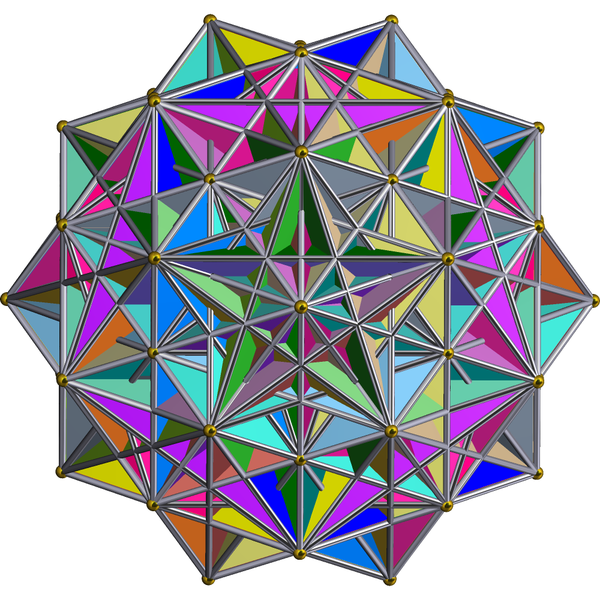
\includegraphics[width=0.4\textwidth]{great-grand-120-cell}}
  \smallskip

  \titlepage
}
\frame{\tableofcontents}


\section{Basics}

\subsection{Four dimensions: what is it?}

\begin{frame}{Four dimensions?}
  \only<1>{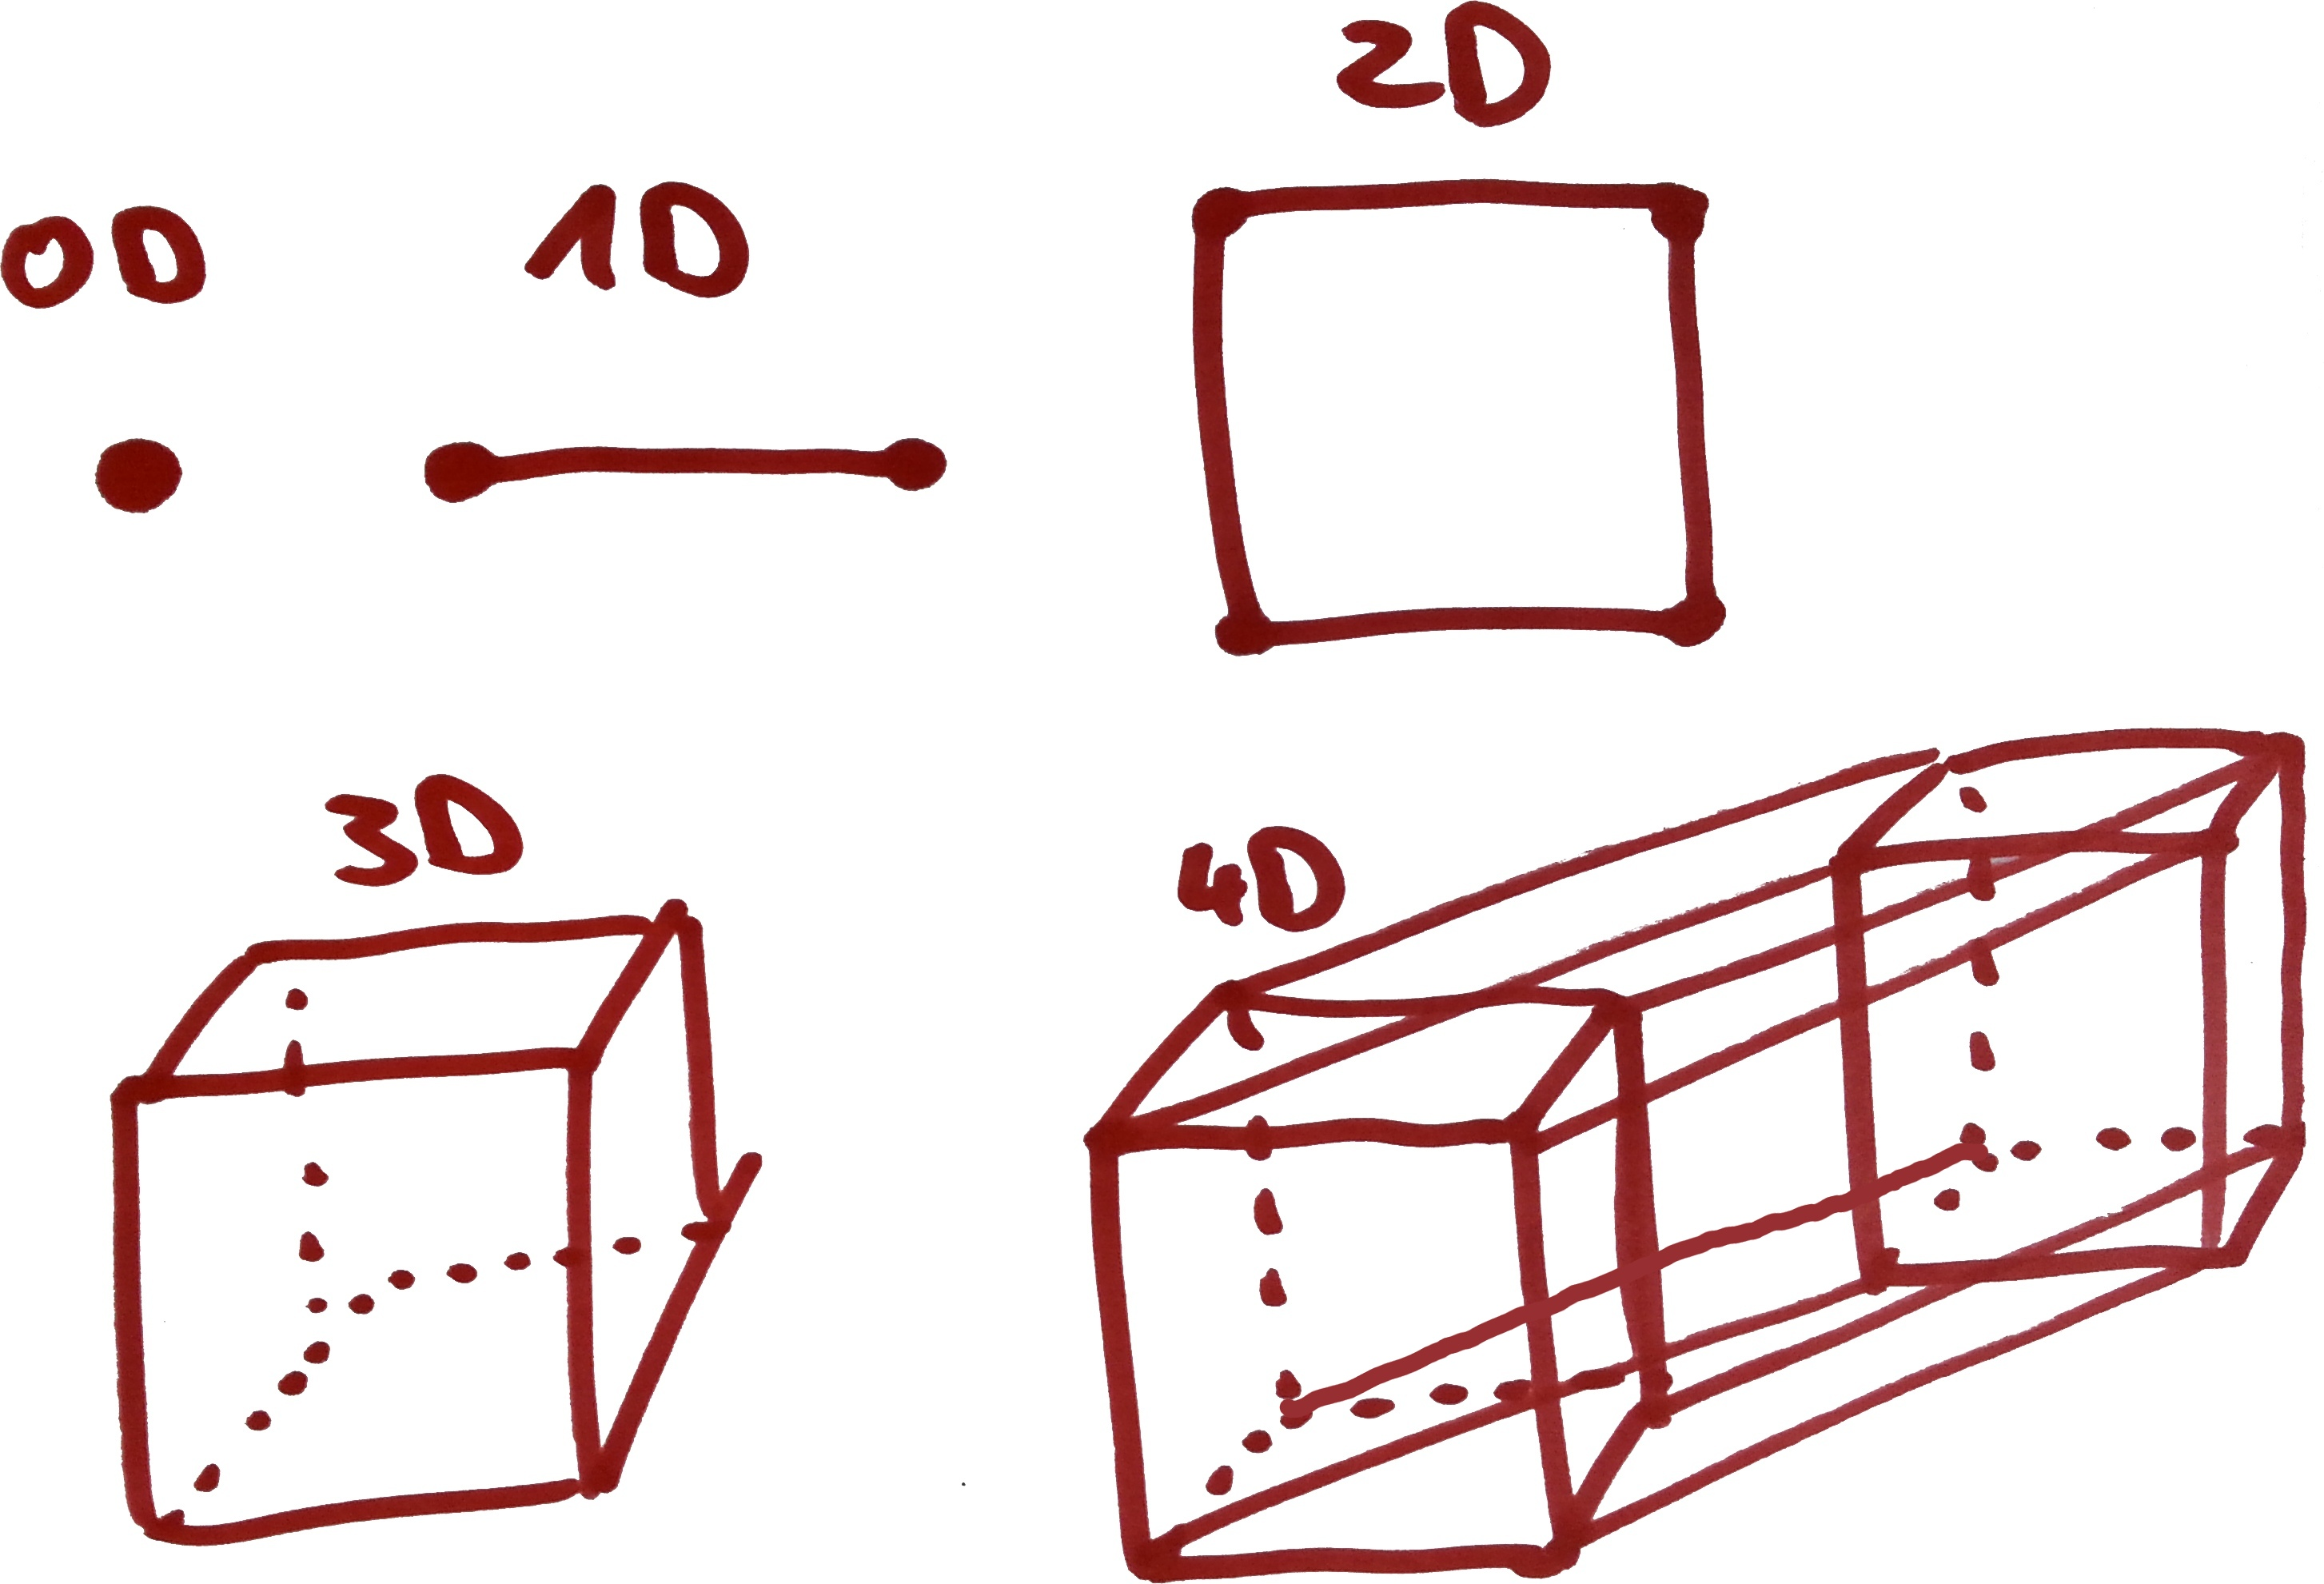
\includegraphics[width=\textwidth]{4d-tesseract}}
  \only<2>{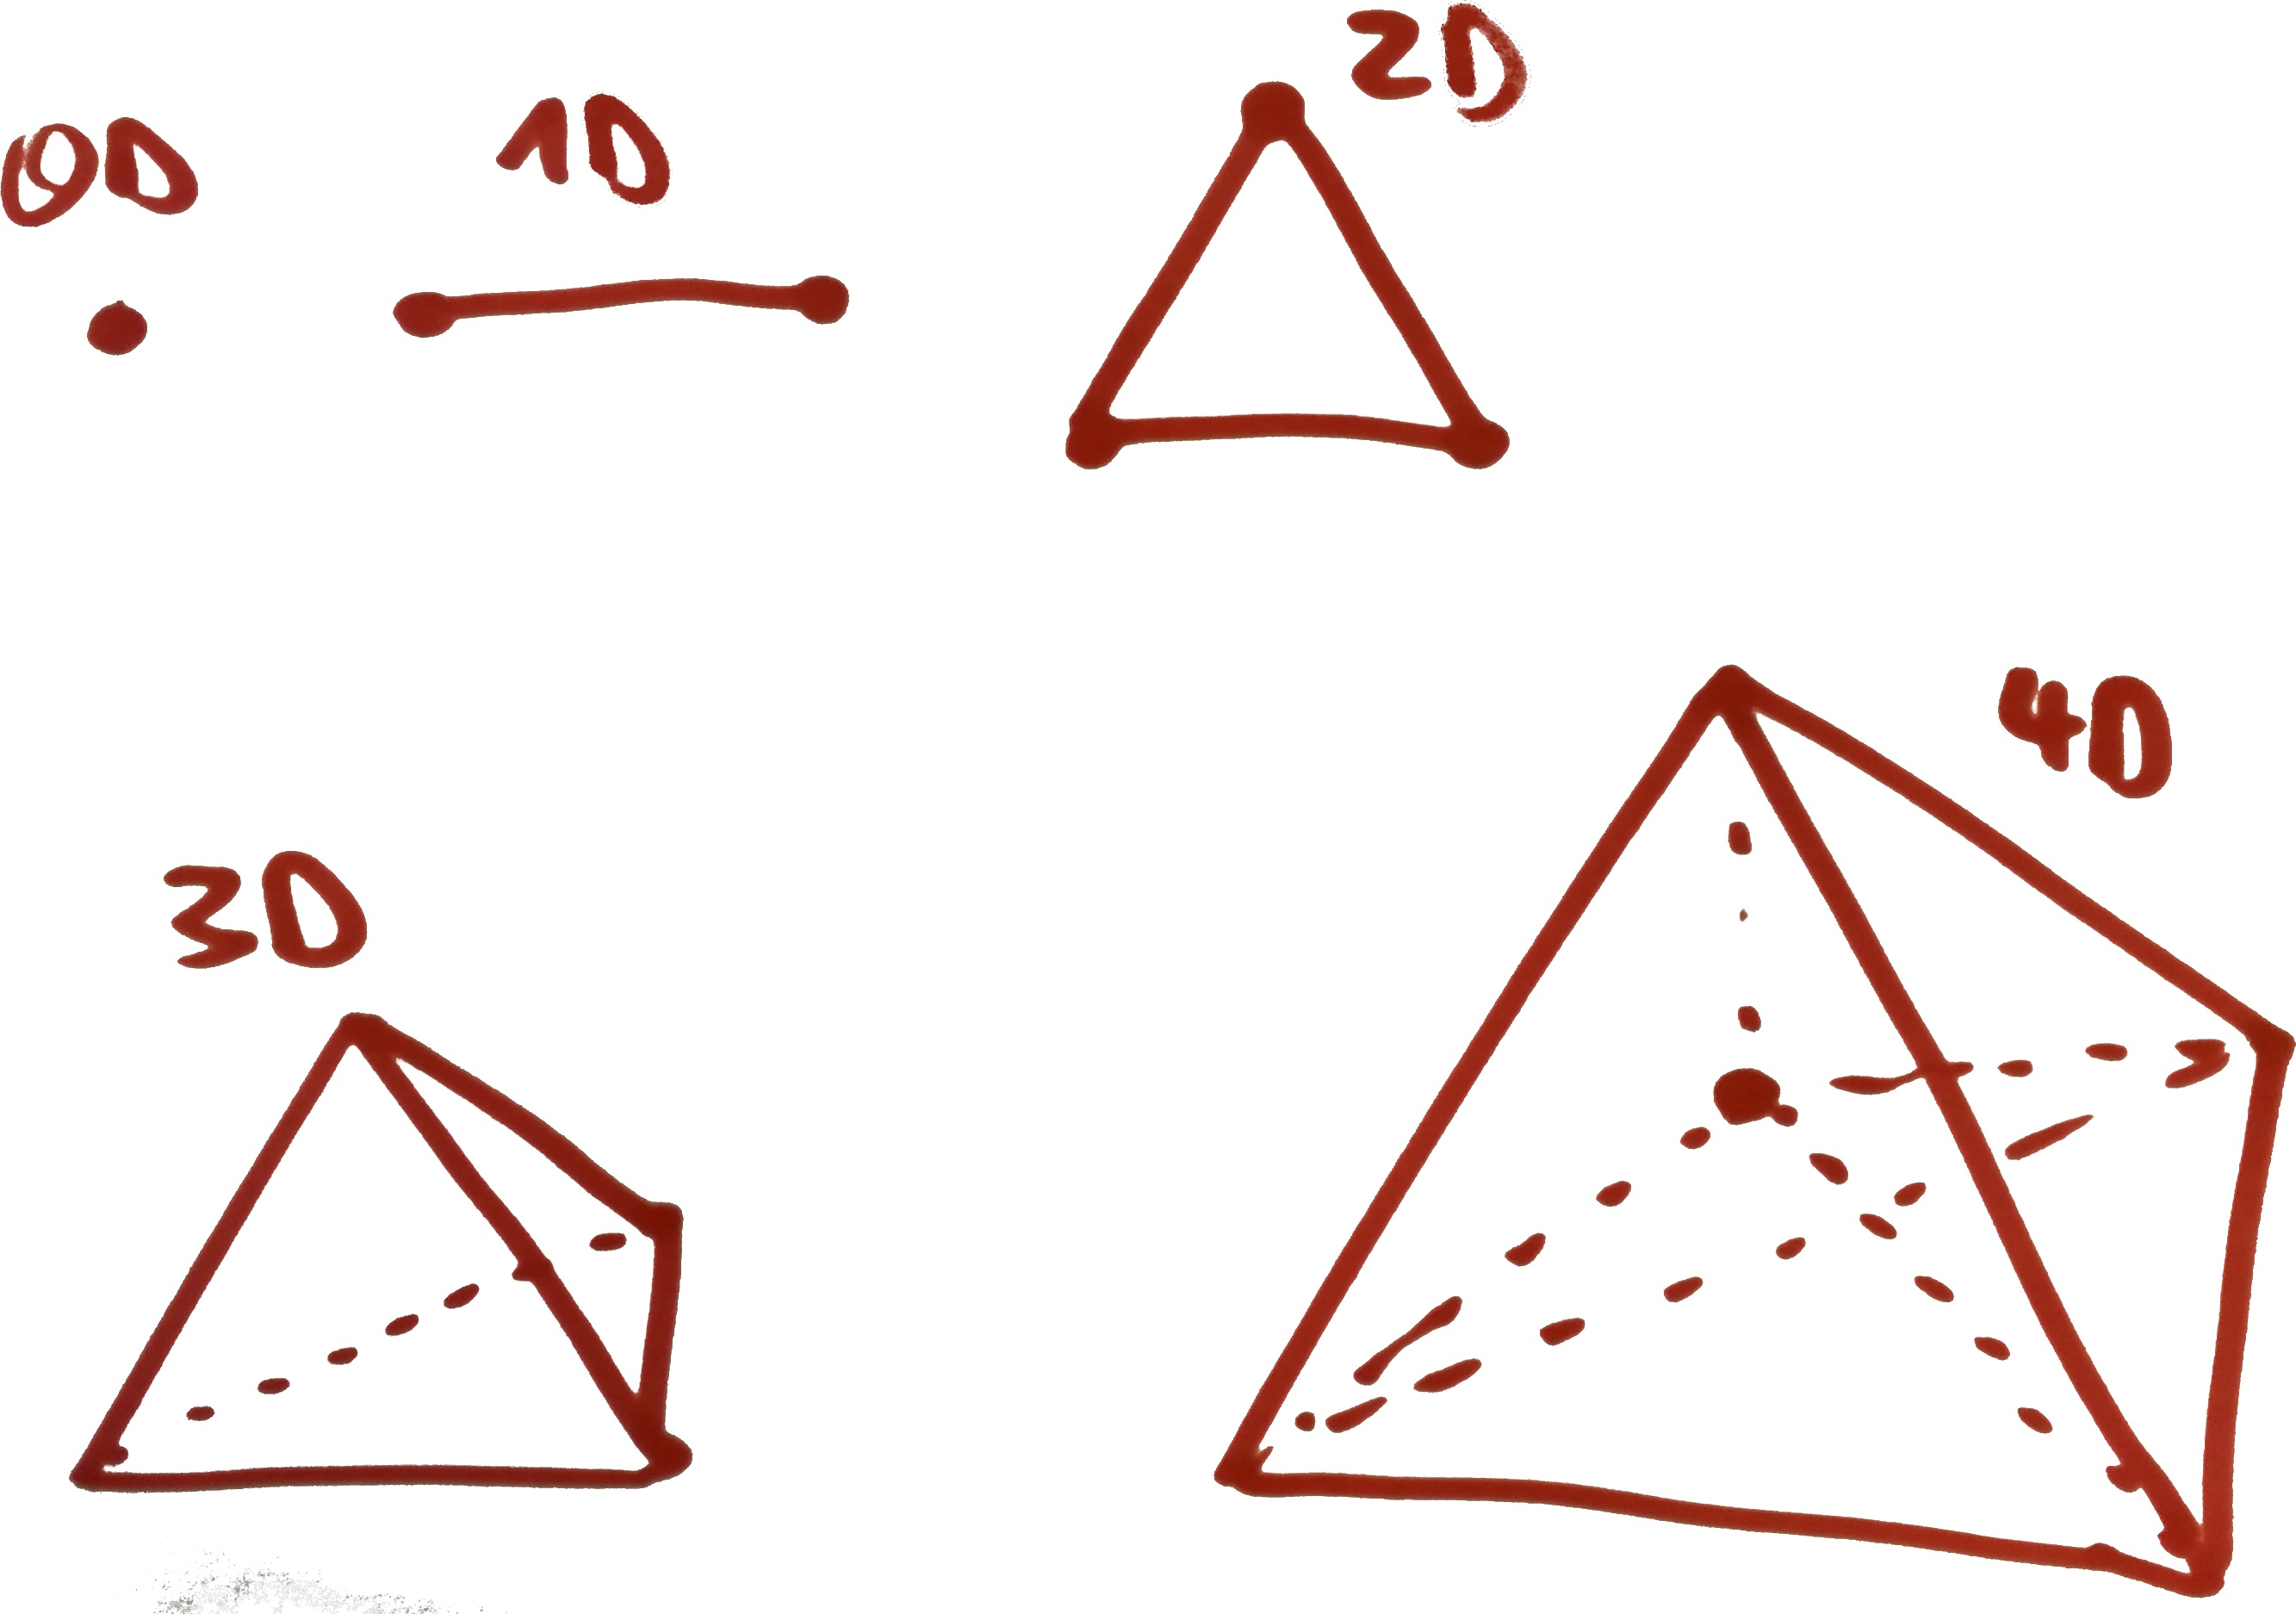
\includegraphics[width=\textwidth]{4d-pentachoron}}
  \only<3>{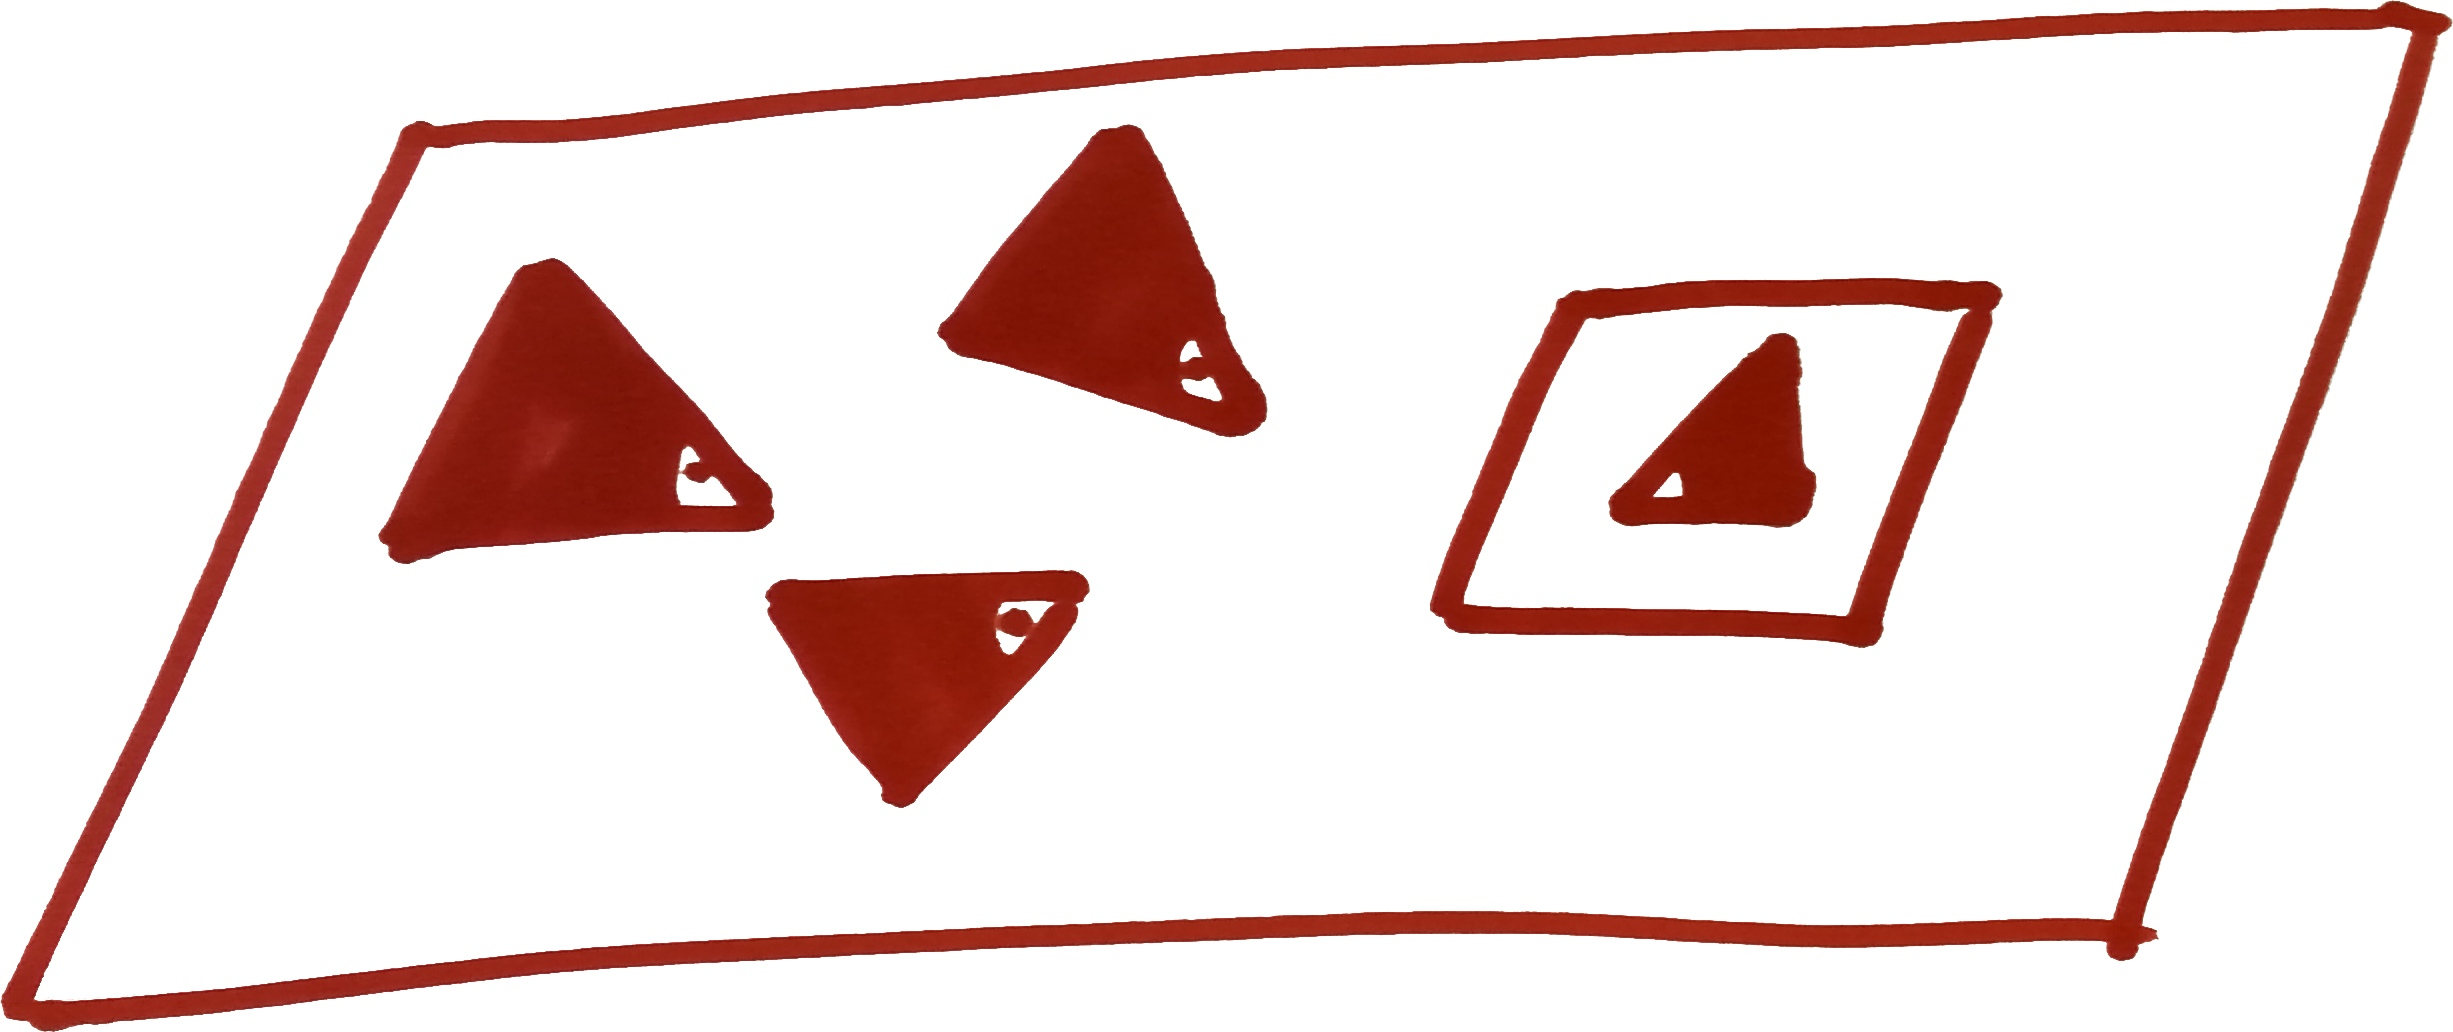
\includegraphics[width=\textwidth]{prisoner}}
  % Skizze Punkt, Linie, Quadrat, Würfel, nach \pause Tesserakt
  % Skizze Punkt, Linie, Dreieck, Tetraeder, 4-dimensionales Simplex
  % Sache mit Projektion erklären
  % klarstellen, dass wir über vierdimensionalen Raum (nicht Raum+Zeit) sprechen
  % nicht: 11-dimensionaler Quantenschaum
  % Wo erkennt man die drei Dimensionen in der realen Welt?
  % Gefängnisse (Quadrat genügt im Flachland, Würfel genügt in 3D, genügt nicht in 4D)
\end{frame}


\subsection{Knot theory}

\begin{frame}{Tieing your shoelaces}
  % Erklären, dass Schnürsenkel immer aufgehen würden
  \centering
  
\includegraphics[width=0.65\textwidth]{trefoil-knot}
  \par
\end{frame}


%Verhedderbar
%in 3D: Schnur, Schnur; 2, 2; 1, 1
%in 3D: Punkt, Fläche;  0, 1; 0, 2
%in 2D: Schnur, Punkt;  1, 2; 1, 0
%in 4D: Schnur, Fläche; 3, 2; 1, 2
%
%Beh.: Dimensionen addiert muss >= n - 1 sein, damit verhedderung möglich ist
%
%Nicht verhedderbar
%in 3D: Punkt, Schnur; 3, 2; 0, 1
%in 3D: Punkt, Punkt;  3, 3; 0, 0
%in 4D: Punkt, Fläche      ; 0, 2
%in 4D: Schnur, Schnur     ; 1, 1

\subsection{The Klein bottle}

\begin{frame}{The Klein bottle}
  \centering
  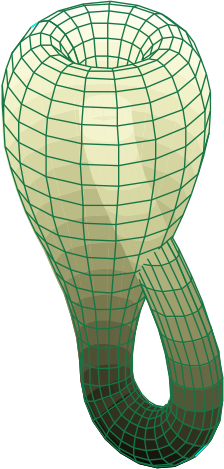
\includegraphics[width=0.75\textwidth]{klein-bottle}
  \par
\end{frame}


\section[Sizes]{Sizes in four dimensions}

\subsection{Hypervolume of hyperspheres}

\begin{frame}{Hypervolume of hyperspheres}
  \centering
  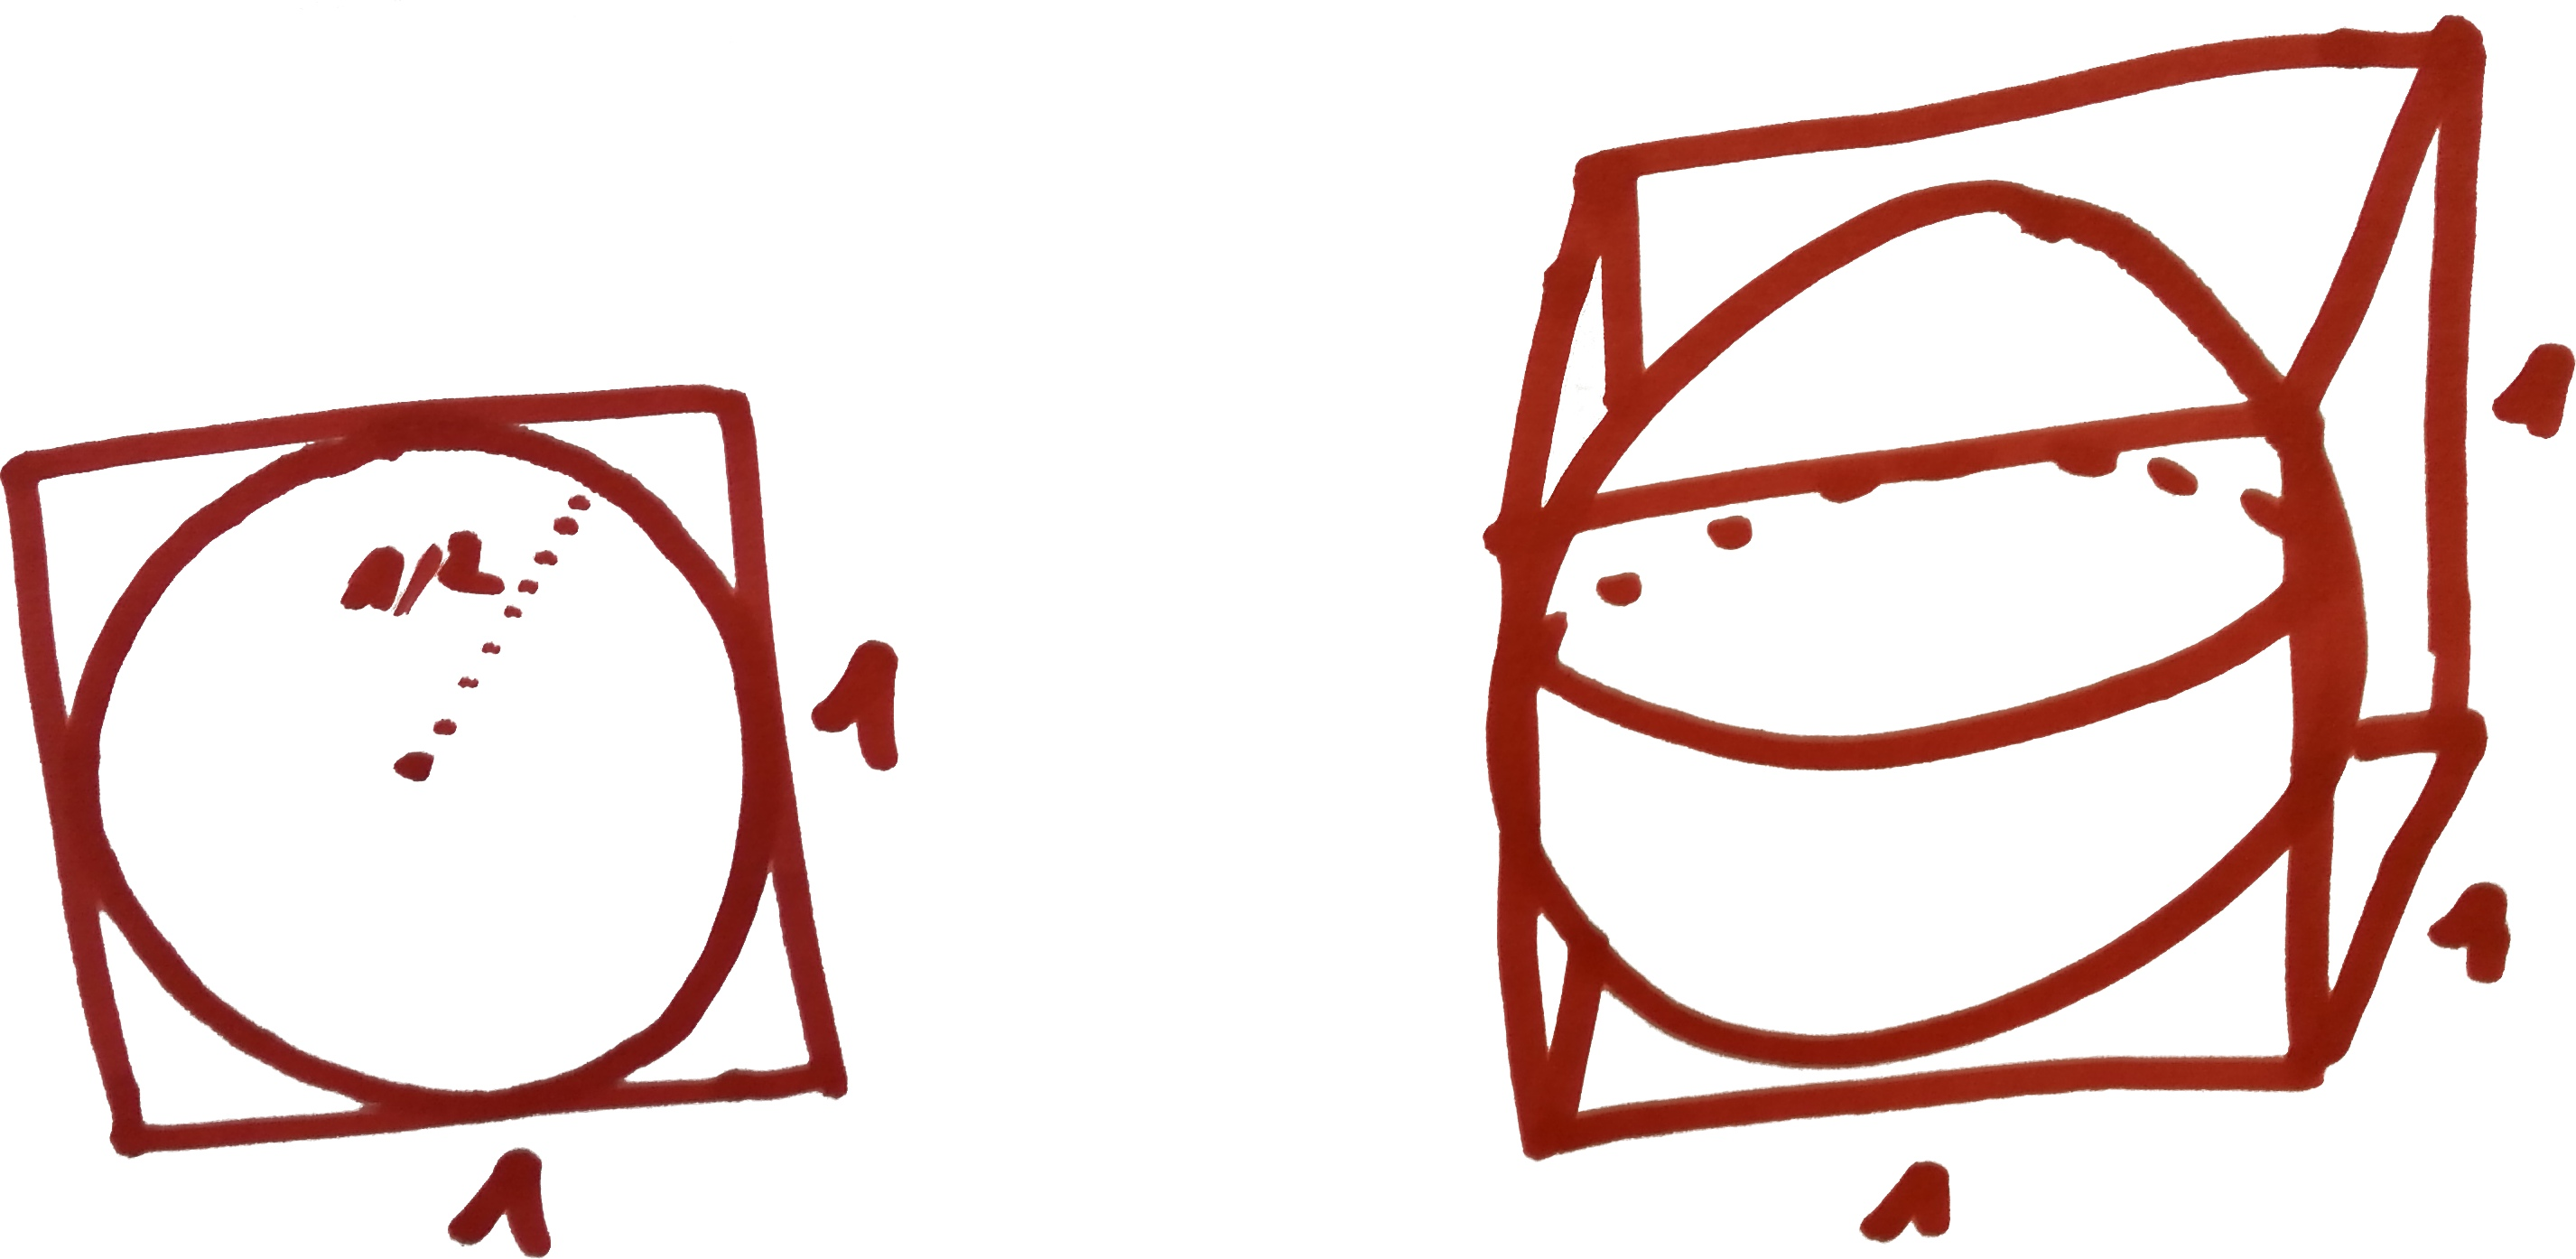
\includegraphics[width=0.4\textwidth]{sizes-1}
  % vorher gscheite Definition der Hyperkugel
  % Bild vom Kreis im Quadrat
  % Bild vom Zylinder im Würfel
  % Bild von der Kugel im Würfel

  \begin{tabular}{lll}
    \toprule
    dimension & hypervolume & \\\midrule
    \only<2>{%
      $n = 0$ & $1$ & $\approx 1.000$ \\
      $n = 1$ & $1$ & $\approx 1.000$ \\
    }%
    $n = 2$ & $\pi / 4$ & $\approx 0.785$ \\
    $n = 3$ & $\pi / 6$ & $\approx 0.524$ \\
    $n = 4$ & $\pi^2 / 32$ & $\approx 0.308$ \\
    $n = 5$ & $\pi^2 / 60$ & $\approx 0.164$ \\
    $n = 6$ & $\pi^3 / 384$ & $\approx 0.081$ \\
    $n = 7$ & $\pi^3 / 840$ & $\approx 0.037$ \\
    $n \to \infty$ & $\to 0$ \\
    \bottomrule
  \end{tabular}\par
\end{frame}

% power of negative thinking


\subsection{Kissing hyperspheres}

\begin{frame}[plain,c]
  \centering\Huge
  \scalebox{2.6}{\hil{Love is}} \\[0.6em]
  \scalebox{2.6}{\hil{important.}}

  \bigskip
  \bigskip

  \scalebox{2.6}{\hil{$\boldsymbol{\heartsuit}$}}
  \par
\end{frame}


\begin{frame}{Kissing hyperspheres}
  % Bild vier Kreise an den Ecken des Zweiheitsquadrats und Kreis in der Mitte
  \centering
  \vspace*{-1em}
  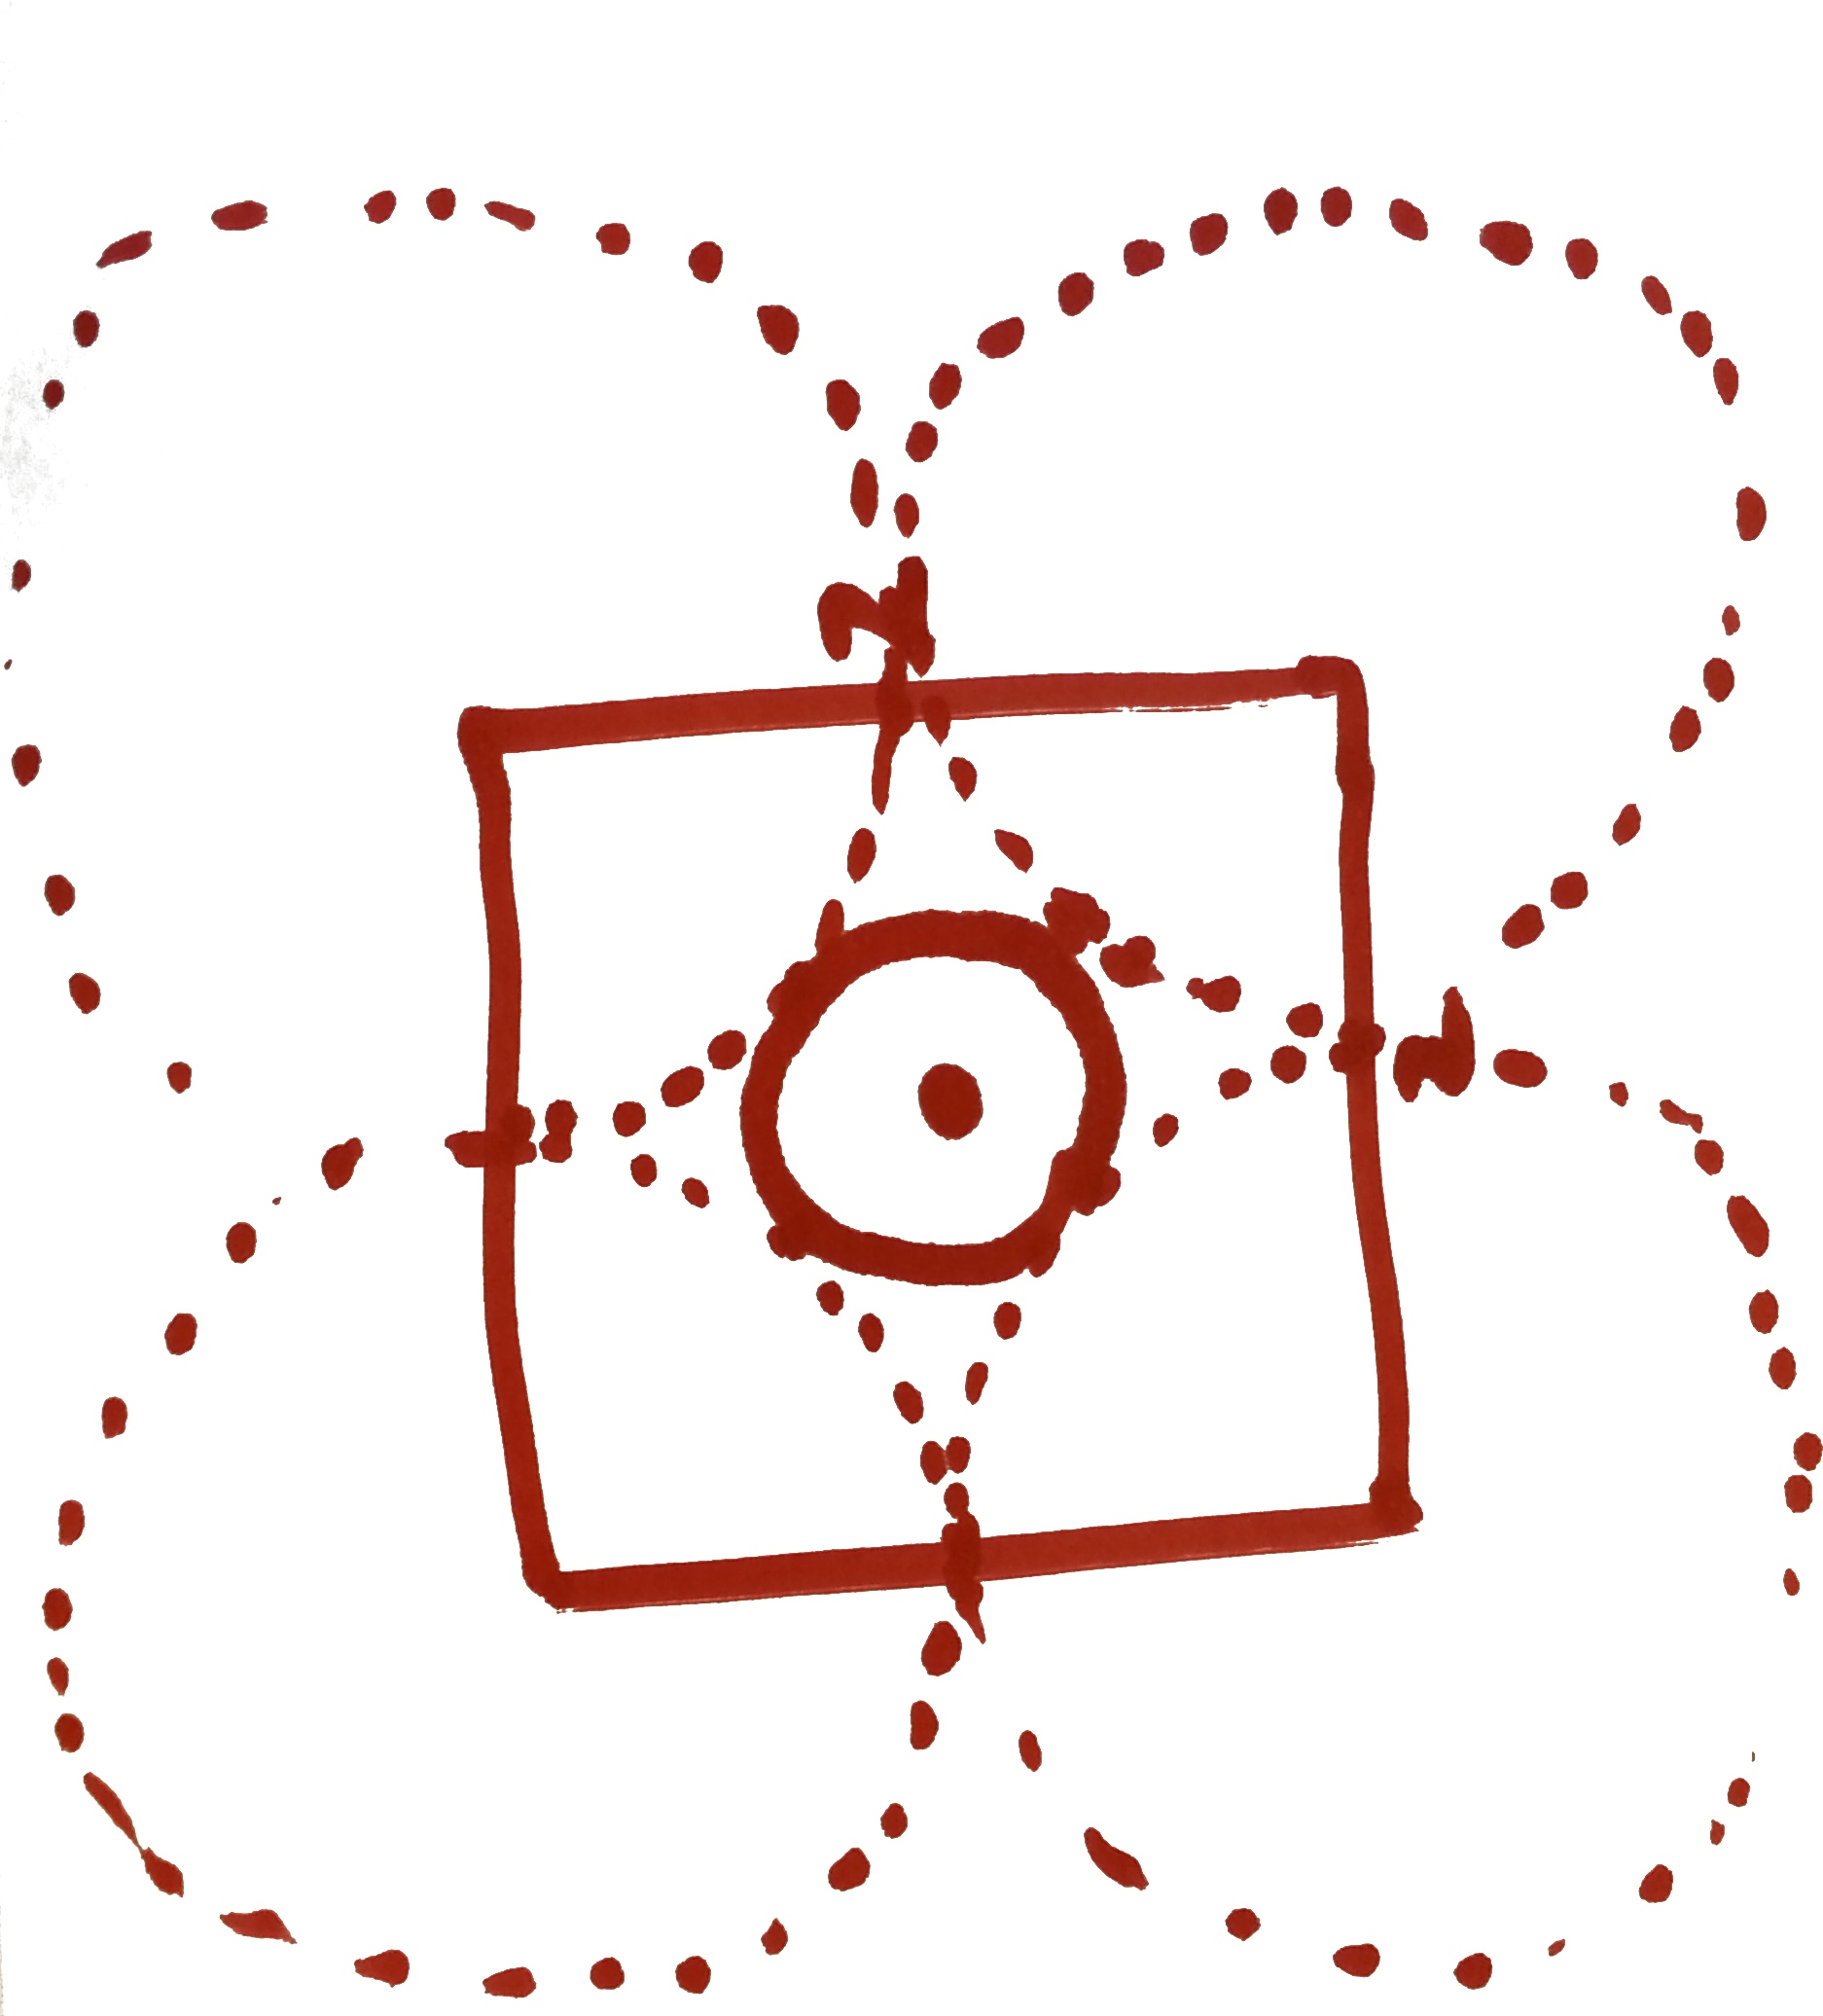
\includegraphics[width=0.3\textwidth]{sizes-2}

  \centering
  \begin{tabular}{lll}
    \toprule
    dimension & radius of the inner hypersphere & \\\midrule
    $n = 2$ & $\sqrt{2} - 1$ \\
    \pause
    $n = 3$ & $\sqrt{3} - 1$ \\
    \pause
    $n = 4$ & $\sqrt{4} - 1$ \\
    \pause
    $n$ & $\sqrt{n} - 1$ \\
    \bottomrule
  \end{tabular}\par
  \bigskip

  \centering
  \hil{The distance to the corners gets bigger and bigger.}
  \par
\end{frame}


\section[Intersection]{Intersection theory}

\subsection{Intersection theory}

\begin{frame}{A hypersphere arrives}
  \centering
  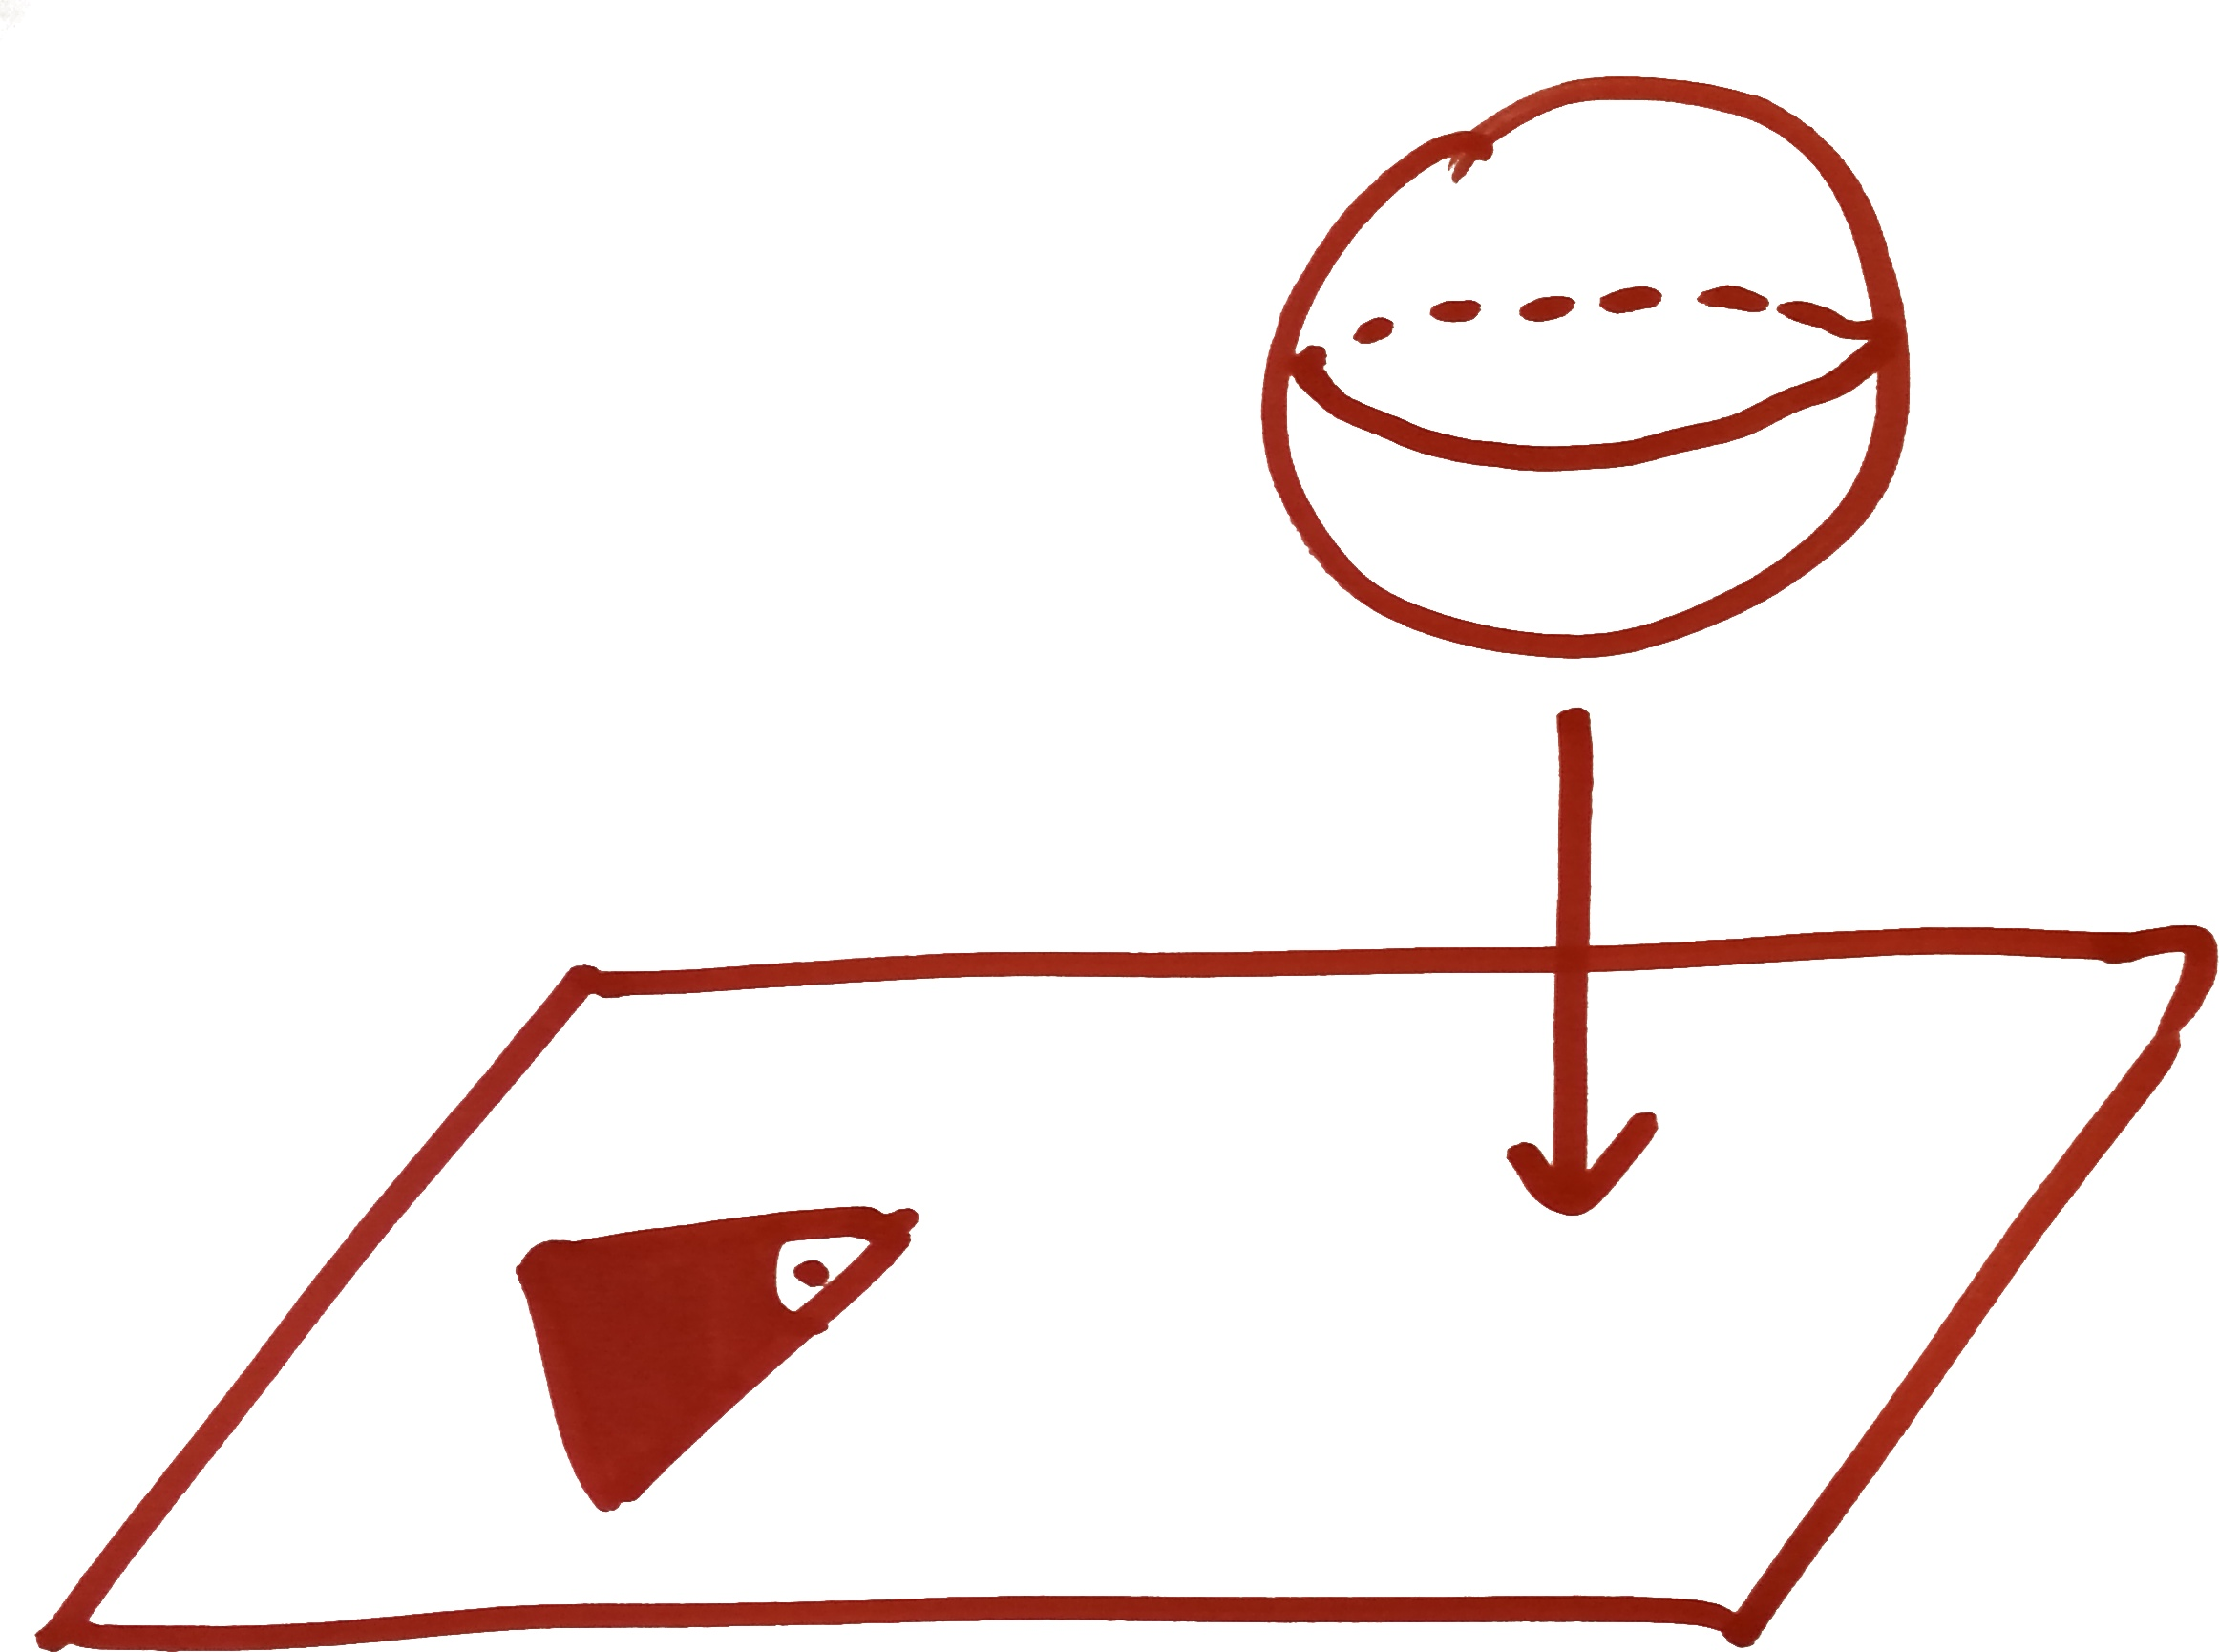
\includegraphics[width=0.9\textwidth]{a-hypersphere-arrives}
  \par
\end{frame}

\begin{frame}{A tesseract arrives}
  \centering
  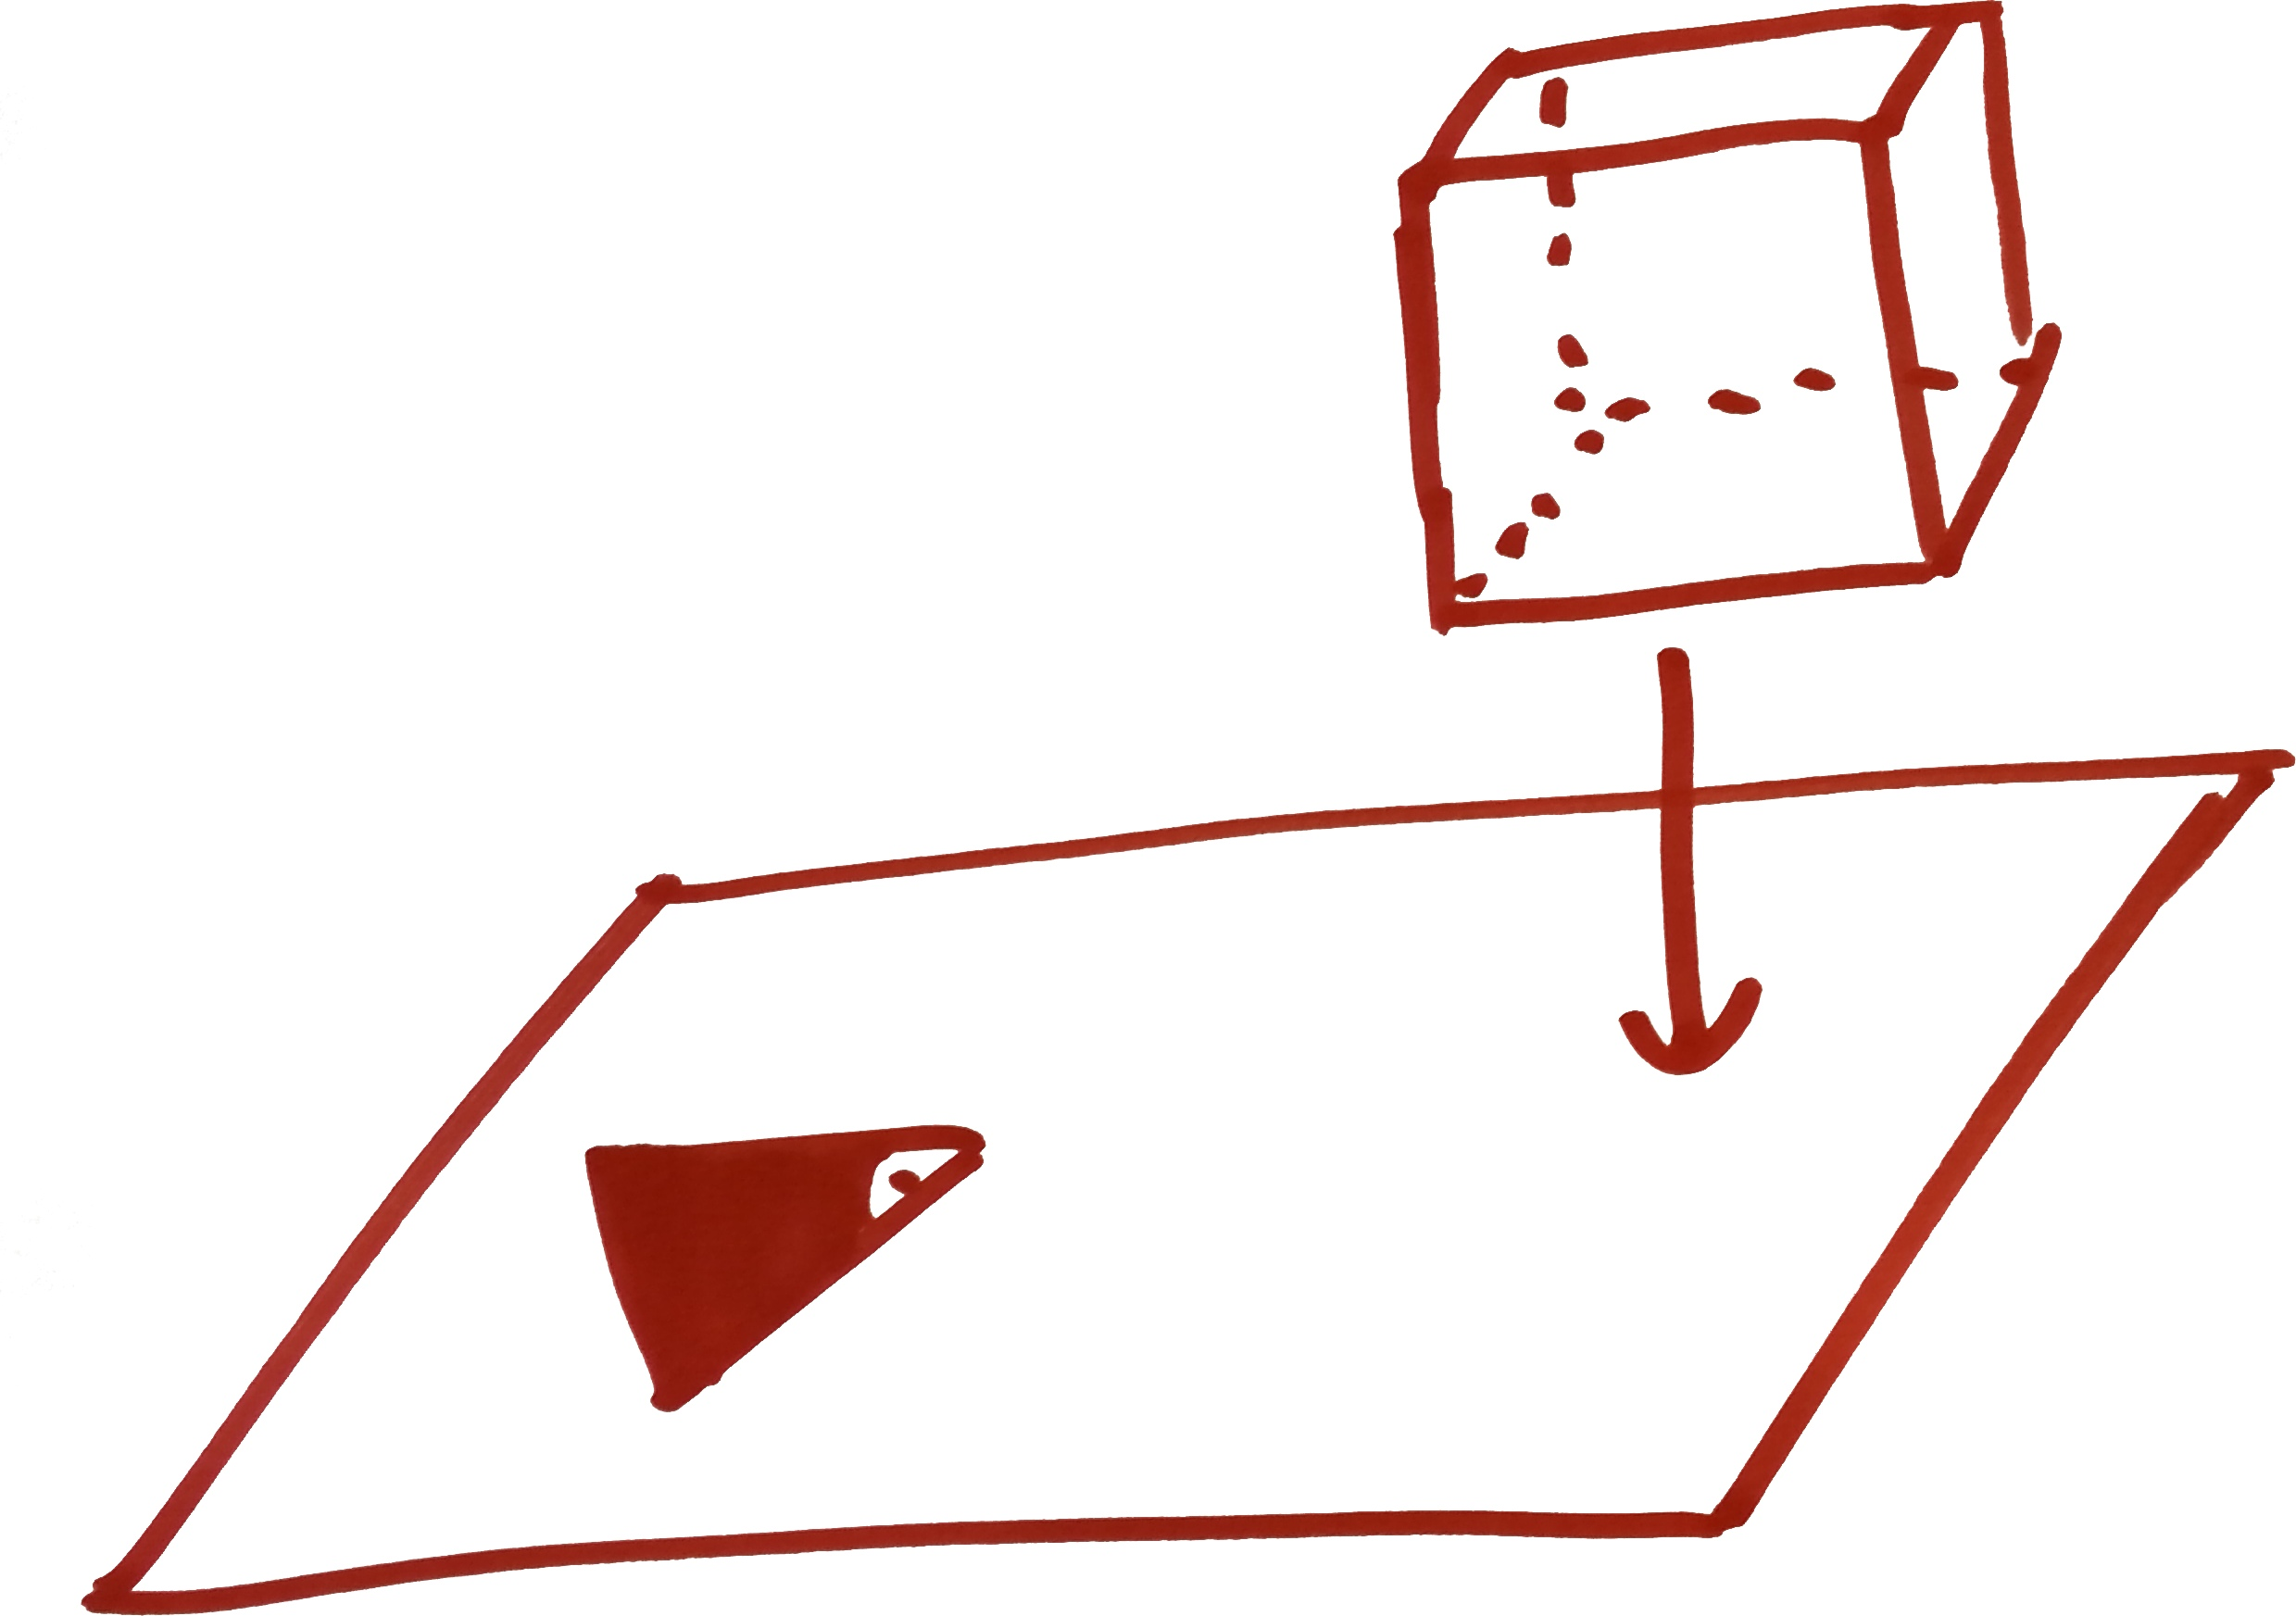
\includegraphics[width=\textwidth]{a-tesseract-arrives}
  \par
\end{frame}



% Jetzt Ecken & Co. zählen

% Tesserakt mit Raum schneiden


\section{Platonic solids}

\newcommand{\solid}[4]{\begin{column}{0.31\textwidth}\centering\hil{#2}\par#3 faces, #4 vertices\\\medskip\includegraphics[height=0.7\textwidth]{#1}\end{column}}
\newcommand{\solidd}[3]{\begin{column}{0.35\textwidth}\centering\hil{#2}\par#3\\\medskip\includegraphics[height=0.6\textwidth]{#1}\end{column}}


\subsection{in 3D}

\begin{frame}{Platonic solids in 3D}
  \begin{columns}[c]
    \solid{tetrahedron}{Tetrahedron}{4}{4}
    \solid{hexahedron}{Hexahedron}{6}{8}
    \solid{octahedron}{Octahedron}{8}{6}
  \end{columns}
  \bigskip
  \begin{columns}[c]
    \solid{dodecahedron}{Dodecahedron}{12}{20}
    \solid{icosahedron}{Icosahedron}{20}{12}
  \end{columns}
\end{frame}


\subsection{in 4D}

\begin{frame}{Platonic solids in 4D}
  \begin{columns}[c]
    \solidd{005-cell}{Pentachoron}{5v, 10e, 10f, 5c}
    \solidd{008-cell}{Octachoron}{16v, 32e, 24f, 8c}
    \solidd{016-cell}{Hexadecahedron}{8v, 24e, 32f, 16c}
  \end{columns}
  \bigskip
  \bigskip
  \begin{columns}[c]
    \solidd{024-cell}{Icositetrachoron}{24v, 96e, 96f, 24c}
    \solidd{120-cell}{Hecatonicosachoron}{600v, 1200e, 720f, 120c}
    \only<2>{\solidd{600-cell}{Hexacosichoron}{120v, 720e, 1200f, 600c}}
  \end{columns}
\end{frame}


% Gravitation

% Verkleben am Ende

\section[Glueing]{Glueing four-dimensional shapes}

\begin{frame}{Glueing four-dimensional shapes}
  \centering
  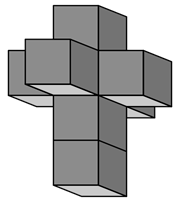
\includegraphics[width=0.6\textwidth]{tesseract-net}
  \par
\end{frame}

\end{document}

Namen für Bewegung in w-Richtung nachschauen
Würfelnetz auf Englisch
Wie man ihn zeichnet (schon zu Beginn)
Fraktale



Ecken:     2 4  8 16
Kanten:    1 4 12 32    32 = (16 * 4) / 2    12 = (8 * 3) / 2
Flächen:   0 1  6 24    (3über2)*8/4 = 6     (4über2)*16/4 = 24 = 2^2 * (4über2)
Volumina:  0 0  1  8
4-Vol.:    0 0  0  1
